\documentclass{beamer}
\mode<presentation>{\usefonttheme{serif}}
\beamertemplatenavigationsymbolsempty
\usetheme{metropolis}
%\usefonttheme[onlymath]{serif}

\usepackage[utf8]{inputenc}
\usepackage{bbm}
\usepackage{amssymb}
\usepackage[absolute,overlay]{textpos}
\usepackage{graphicx}
\usepackage{tikz}
\usepackage{courier}

\title{
	{{\Large \textbf{Encontros Matemáticos}} {\small 	apresenta}}\\
\vspace{30pt}
\texttt{\huge Computação Quântica}
}
\institute{IM-UFRJ}
\date{19 de novembro de 2019}

\author{Pedro Maciel Xavier \\ \texttt{pedromxavier@poli.ufrj.br}}

\newcommand{\teorema}[1]{%
	\textbf{Teorema. (\emph{#1})\\}
}

\newcommand{\prova}{%
	\textbf{Prova.\\}
}

\newcommand{\cqd}{%
	{\flushright \blacksquare\\}
}

\newcommand{\postulado}[1]{%
	\textbf{Postulado. (\emph{#1})\\}
}

\newcommand{\definicao}[1]{%
	\textbf{Definição. (\emph{#1})\\}
}

\newcommand{\vetor}[2]{\ensuremath{
\left[\begin{matrix}
#1 \\
#2
\end{matrix}\right]
}
}

\newcommand{\vetorx}[4]{\ensuremath{
\left[\begin{matrix}
#1 \\
#2 \\
#3 \\
#4
\end{matrix}\right]
}
}

\newcommand{\ket}[1]{\ensuremath{\left|#1\right\rangle}}
\newcommand{\bra}[1]{\ensuremath{\left\langle|#1\right|}}

\newcommand{\braket}[2]{\ensuremath{\left\langle#1|#2\right\rangle}}

\newcommand{\ketbra}[2]{\ensuremath{\left|#1\right\rangle\left\langle#2\right|}}

\newcommand{\comich}[1]{
	\bgroup
	\setbeamercolor{background canvas}{bg=white}
	\begin{frame}[plain]{}
		\begin{center}
			\begin{figure}
				\includegraphics[height=\textheight]{#1}
			\end{figure}
		\end{center}
	\end{frame}
	\egroup
}

\newcommand{\comic}[1]{\comich{#1}}

\newcommand{\comicw}[1]{
	\bgroup
	\setbeamercolor{background canvas}{bg=white}
	\begin{frame}[plain]{}
	\begin{center}
		\begin{figure}
			\includegraphics[width=\textwidth]{#1}
		\end{figure}
	\end{center}
\end{frame}
\egroup
}

\newcommand{\comicfinal}[1]{
	\bgroup
	\usebackgroundtemplate{\includegraphics[width=\paperwidth]{#1}}
	\begin{frame}[plain]{}

	\end{frame}
	\egroup
}

\newcommand{\person}[6]{%
% image, name, comment,
% size, dx, dy
\begin{textblock*}{#4}(#5, #6)
	\includegraphics[width=#4]{#1}\\
	#2\\
	{\small #3}
\end{textblock*}
}

\newcommand{\imgw}[2]{%
\begin{center}
	\begin{figure}
	\includegraphics[width=#2]{#1}\\
	\end{figure}
\end{center}
}

\newcommand{\imgh}[2]{%
\begin{center}
	\begin{figure}
		\includegraphics[height=#2]{#1}\\
	\end{figure}
\end{center}
}

\begin{document}

	\begin{frame}
		\titlepage
	\end{frame}
	
	\begin{frame}{Parte I}
  		\tableofcontents[sections={1}]
    \end{frame}

    \begin{frame}{Parte II}
  		\tableofcontents[sections={2-4}]
	\end{frame}

    \begin{frame}{Parte III}
  		\tableofcontents[sections={5-}]
	\end{frame}
	
	\comich{bits0.pdf}
	\comich{bits1.pdf}
	\comich{bits2.pdf}
	\comich{bits3.pdf}
	\comich{bits4.pdf}
	\comicfinal{blue-screen.pdf}

	\section{Computação Digital}
	
	\subsection{bits}
	
	\begin{frame}{\subsecname}
	
	\vspace{-90pt}
	
	Sobre os \textit{bits}:
		\begin{itemize}
			\item Eles moram em $\mathbb{Z}_2$
			\item Realizamos operações \textit{Booleanas} com eles: $\neg$, $\wedge$, $\vee$, $\oplus$.
			\item Formam vetores em $\mathbb{Z}_2^n$, onde cada $\vec{a} = (a_1, a_2, \dots, a_n) \in \mathbb{Z}_2^n$ representa um valor entre $00...0 = 0$ e $11...1 = 2^n-1$.
			
		\end{itemize}
	\end{frame}
	
	\subsection{Álgebra Booleana}
	
	\begin{frame}{\subsecname}
		\person{boole.jpg}{George Boole}{1815 - 1864}{3cm}{2cm}{2cm}
		\person{de-morgan.jpg}{Augustus De Morgan}{1806 - 1871}{4cm}{8cm}{2cm}

	\end{frame}

	\subsection{Complexidade e Computabilidade}	
	
	\begin{frame}{\subsecname}
		\person{church.jpg}{Alonzo Church}{}{3cm}{2cm}{2cm}
		\person{turing.jpg}{Alan Turing}{}{3cm}{8cm}{2.5cm}
	\end{frame}
	
	\begin{frame}{\subsecname}
		\definicao{Complexidade Assintótica}
		Seja um problema com entrada de tamanho $n$, ...
	\end{frame}


	\comich{first-transistor.pdf}
	
	\subsection{Transistor}	
	
	\begin{frame}{\subsecname}
	
	\end{frame}
	
	\subsection{Portas Lógicas}	
	
	\begin{frame}{\subsecname}
		
		\begin{figure}
			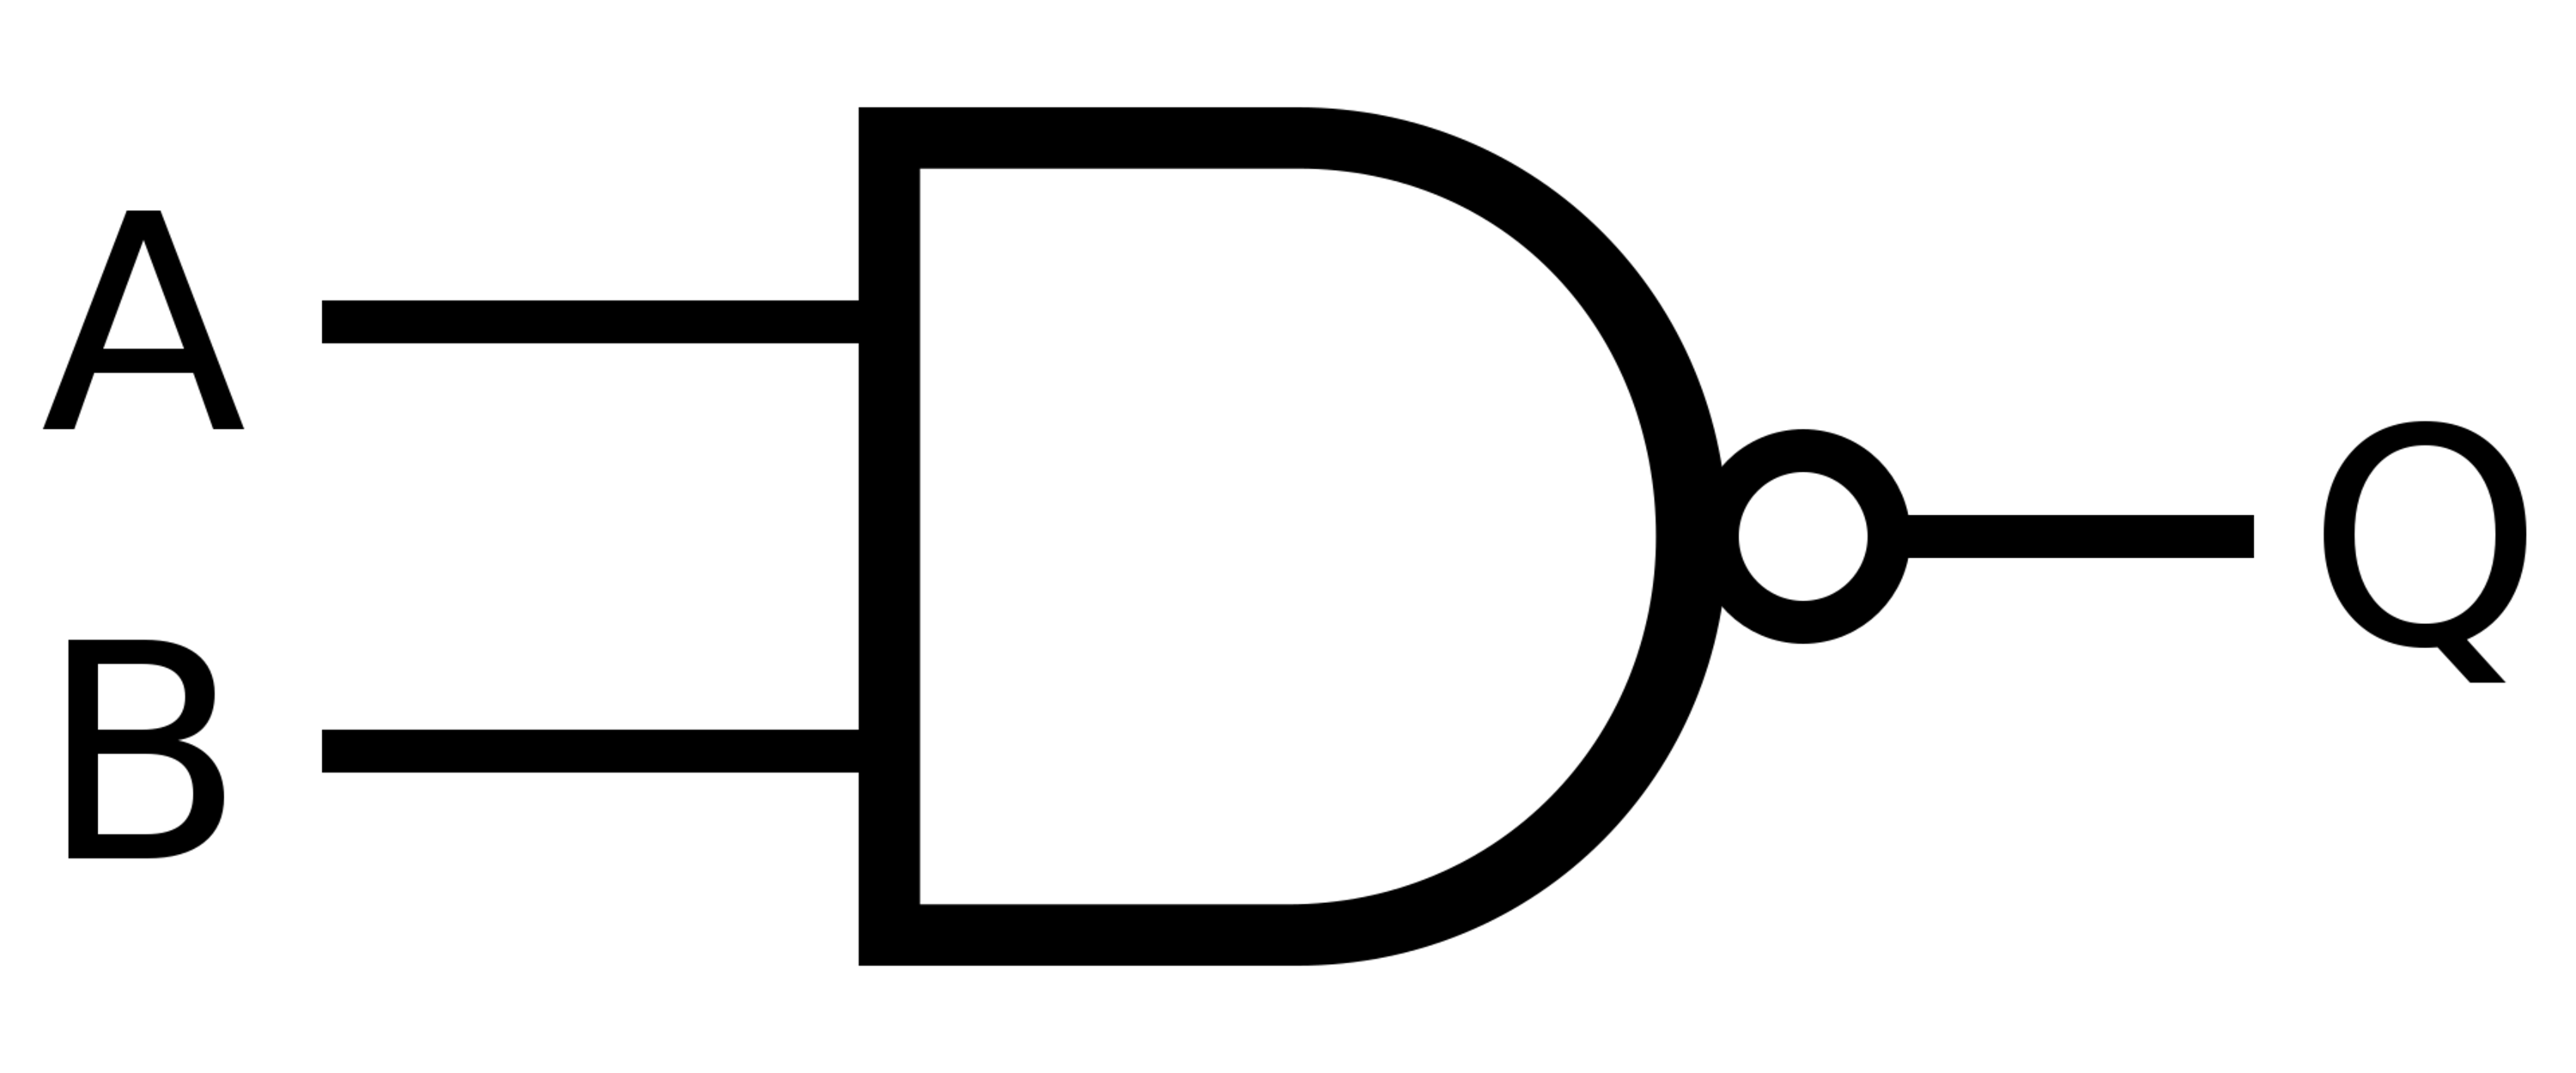
\includegraphics[width=3cm]{nand.pdf}
		\end{figure}
	
	\end{frame}		

	\subsection{Arquitetura de Von Neuman}

	\begin{frame}{\subsecname}
		\person{von-neuman.jpg}{John Von Neuman}{1903 - 1957}{3cm}{2cm}{2cm}
	\end{frame}
		
		
	\subsection{Lei de Moore}
	
	\comicfinal{moores-law.pdf}
	
	\begin{frame}
		\person{moore.jpg}{Gordon Moore}{Intel, 1965}{3cm}{5cm}{3cm}
	\end{frame}

	\begin{frame}{Fenômenos Quânticos}
		\person{feynman.jpg}{Richard Feynman}{1918 - 1988}{3cm}{2cm}{2cm}
			
	\end{frame}
		
	
	\section{Computação Quântica}
	
	\subsection{Postulados}
	
	\begin{frame}{\subsecname}
		\postulado{Representação}
		\begin{align*}
			\ket{\Psi} \in \mathbb{C}^2 && (\mathbf{x} \in \mathbb{C}^2)\\
%%			\braket{\Psi}{\Psi} = 1 (\mathbf{x}^{\dagger} \mathbf{x} = 1)
		\end{align*}
		\vspace{-1cm} 
		\begin{figure}[H]
			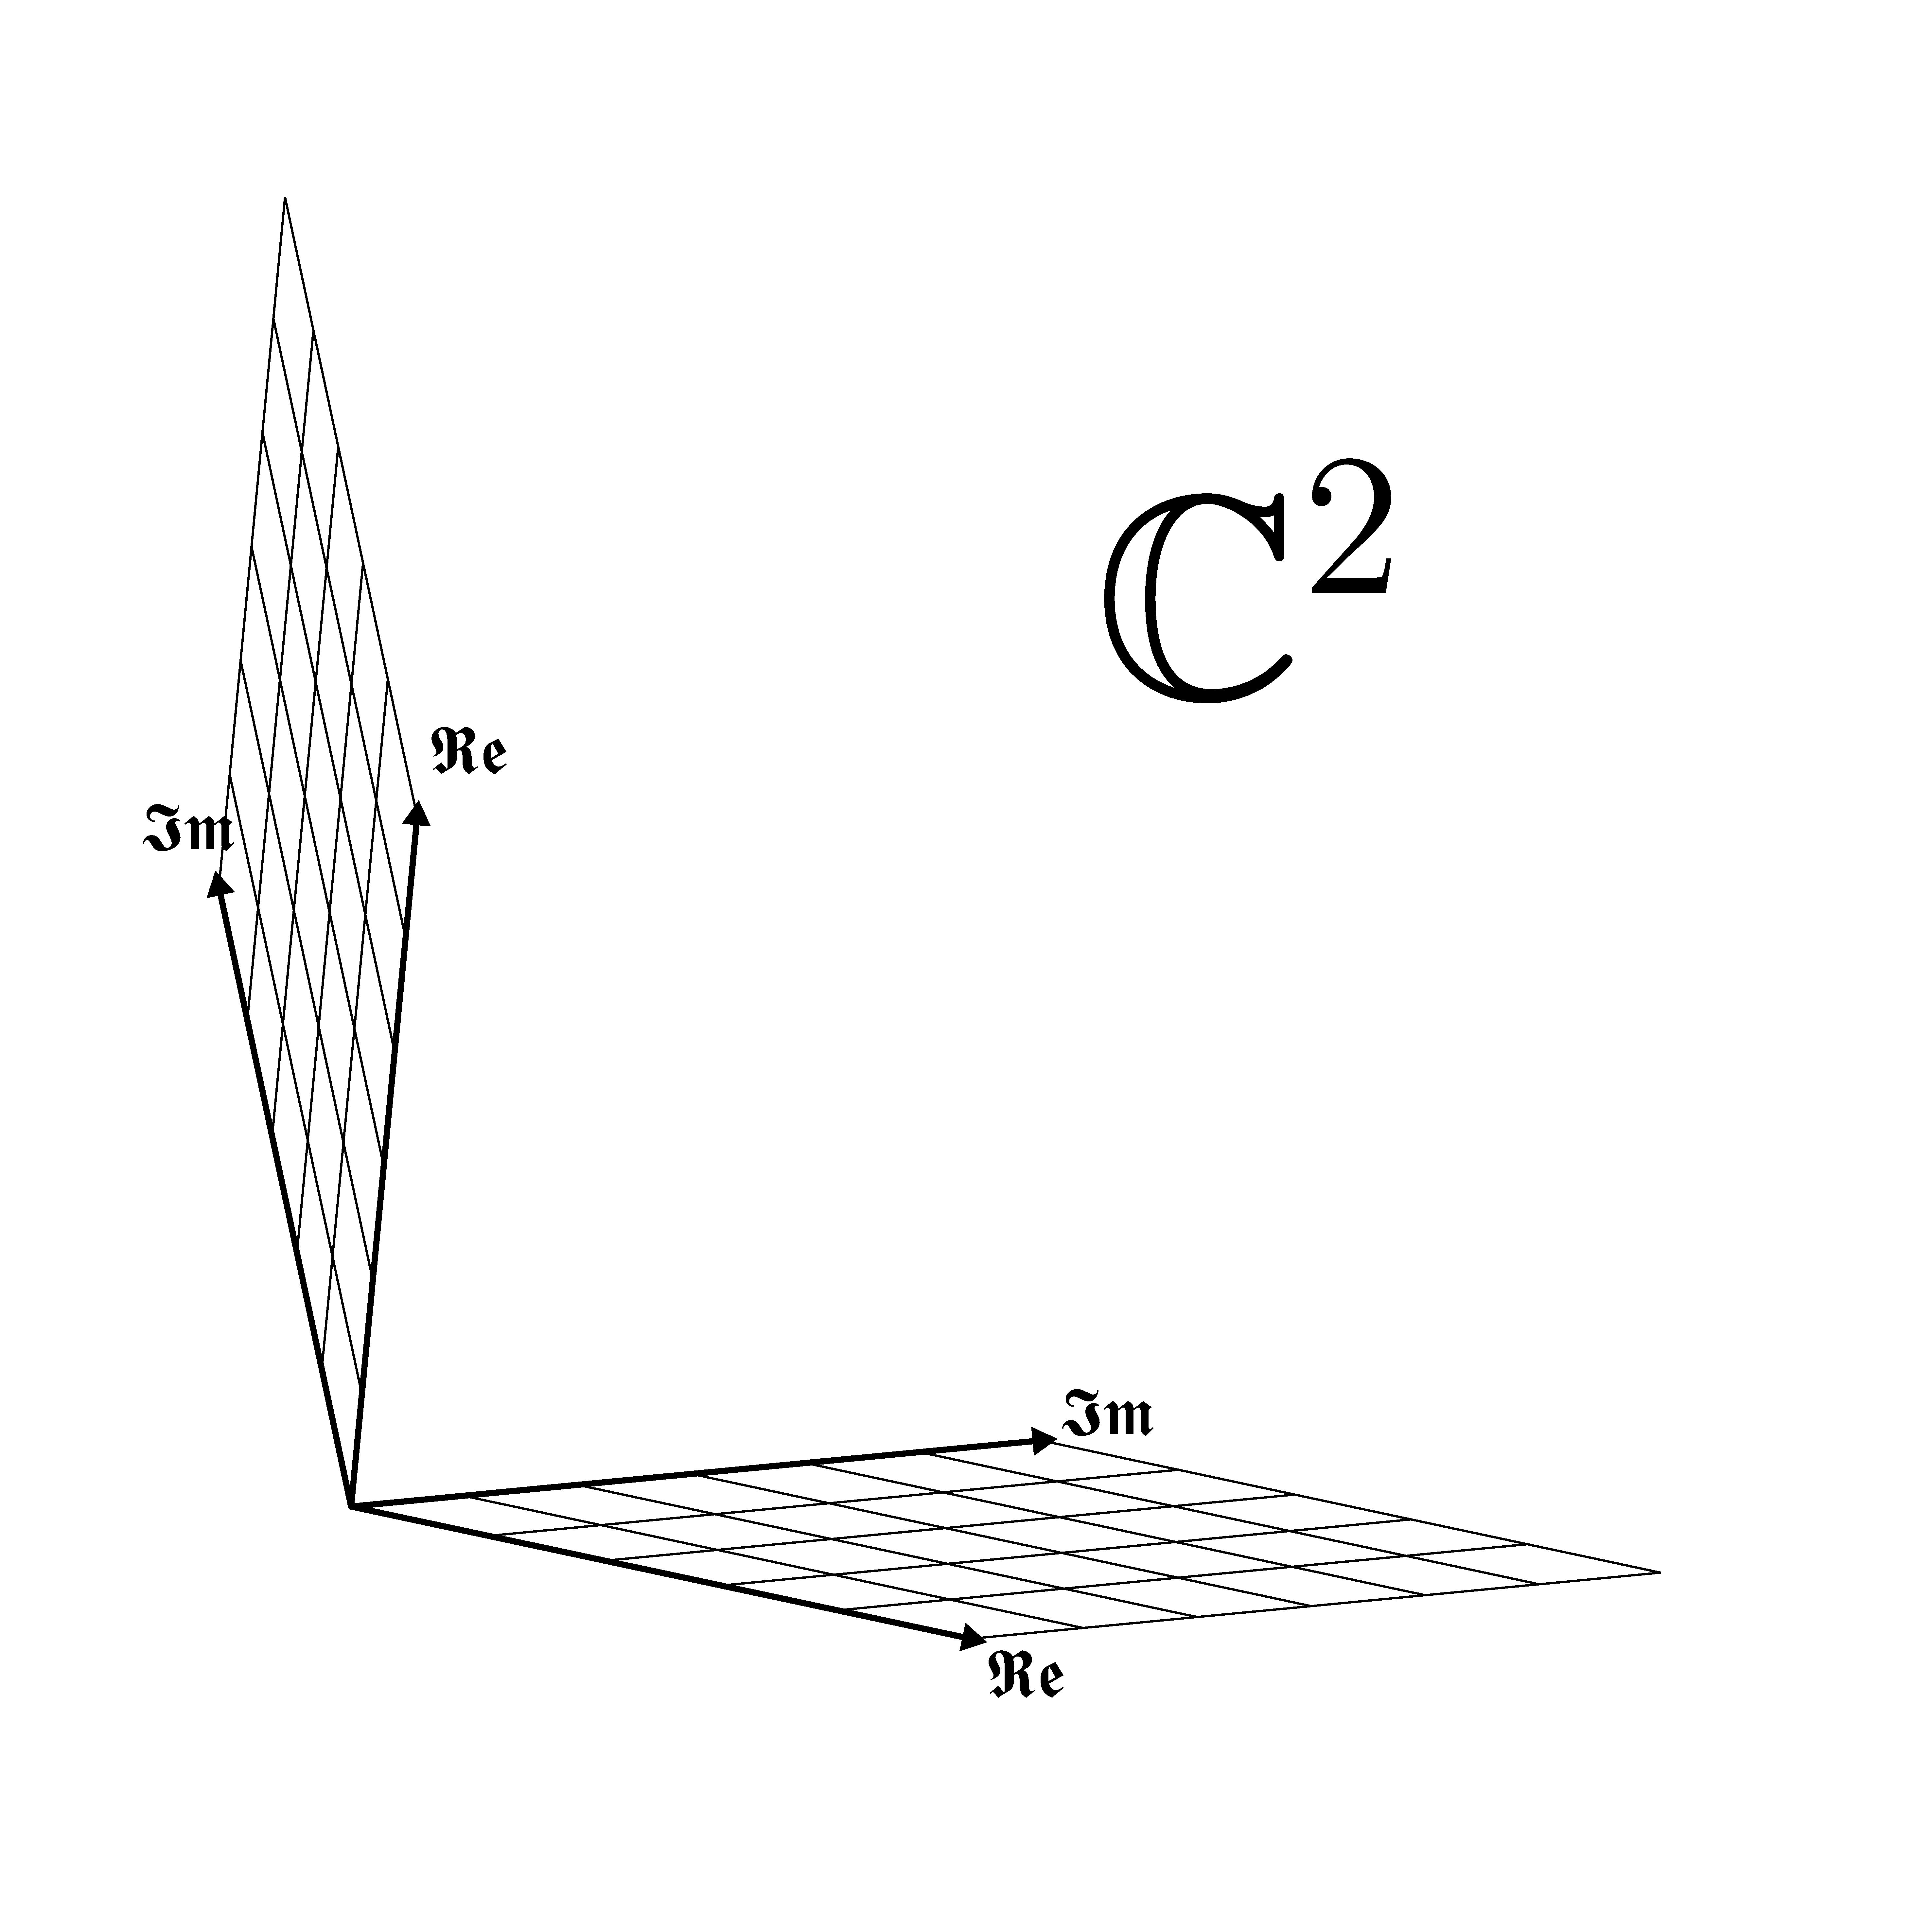
\includegraphics[width=6cm]{c2.pdf}
		\end{figure}
	\end{frame}
	
	\begin{frame}{\subsecname}
		\postulado{Representação}
		\begin{align*}
			\ket{\Psi} \in \mathbb{C}^2 && (\mathbf{x} \in \mathbb{C}^2)\\
			\braket{\Psi}{\Psi} = 1 && (\mathbf{x}^{\dagger} \mathbf{x} = 1)
		\end{align*}
		\vspace{-1cm}
		\begin{figure}[H]
			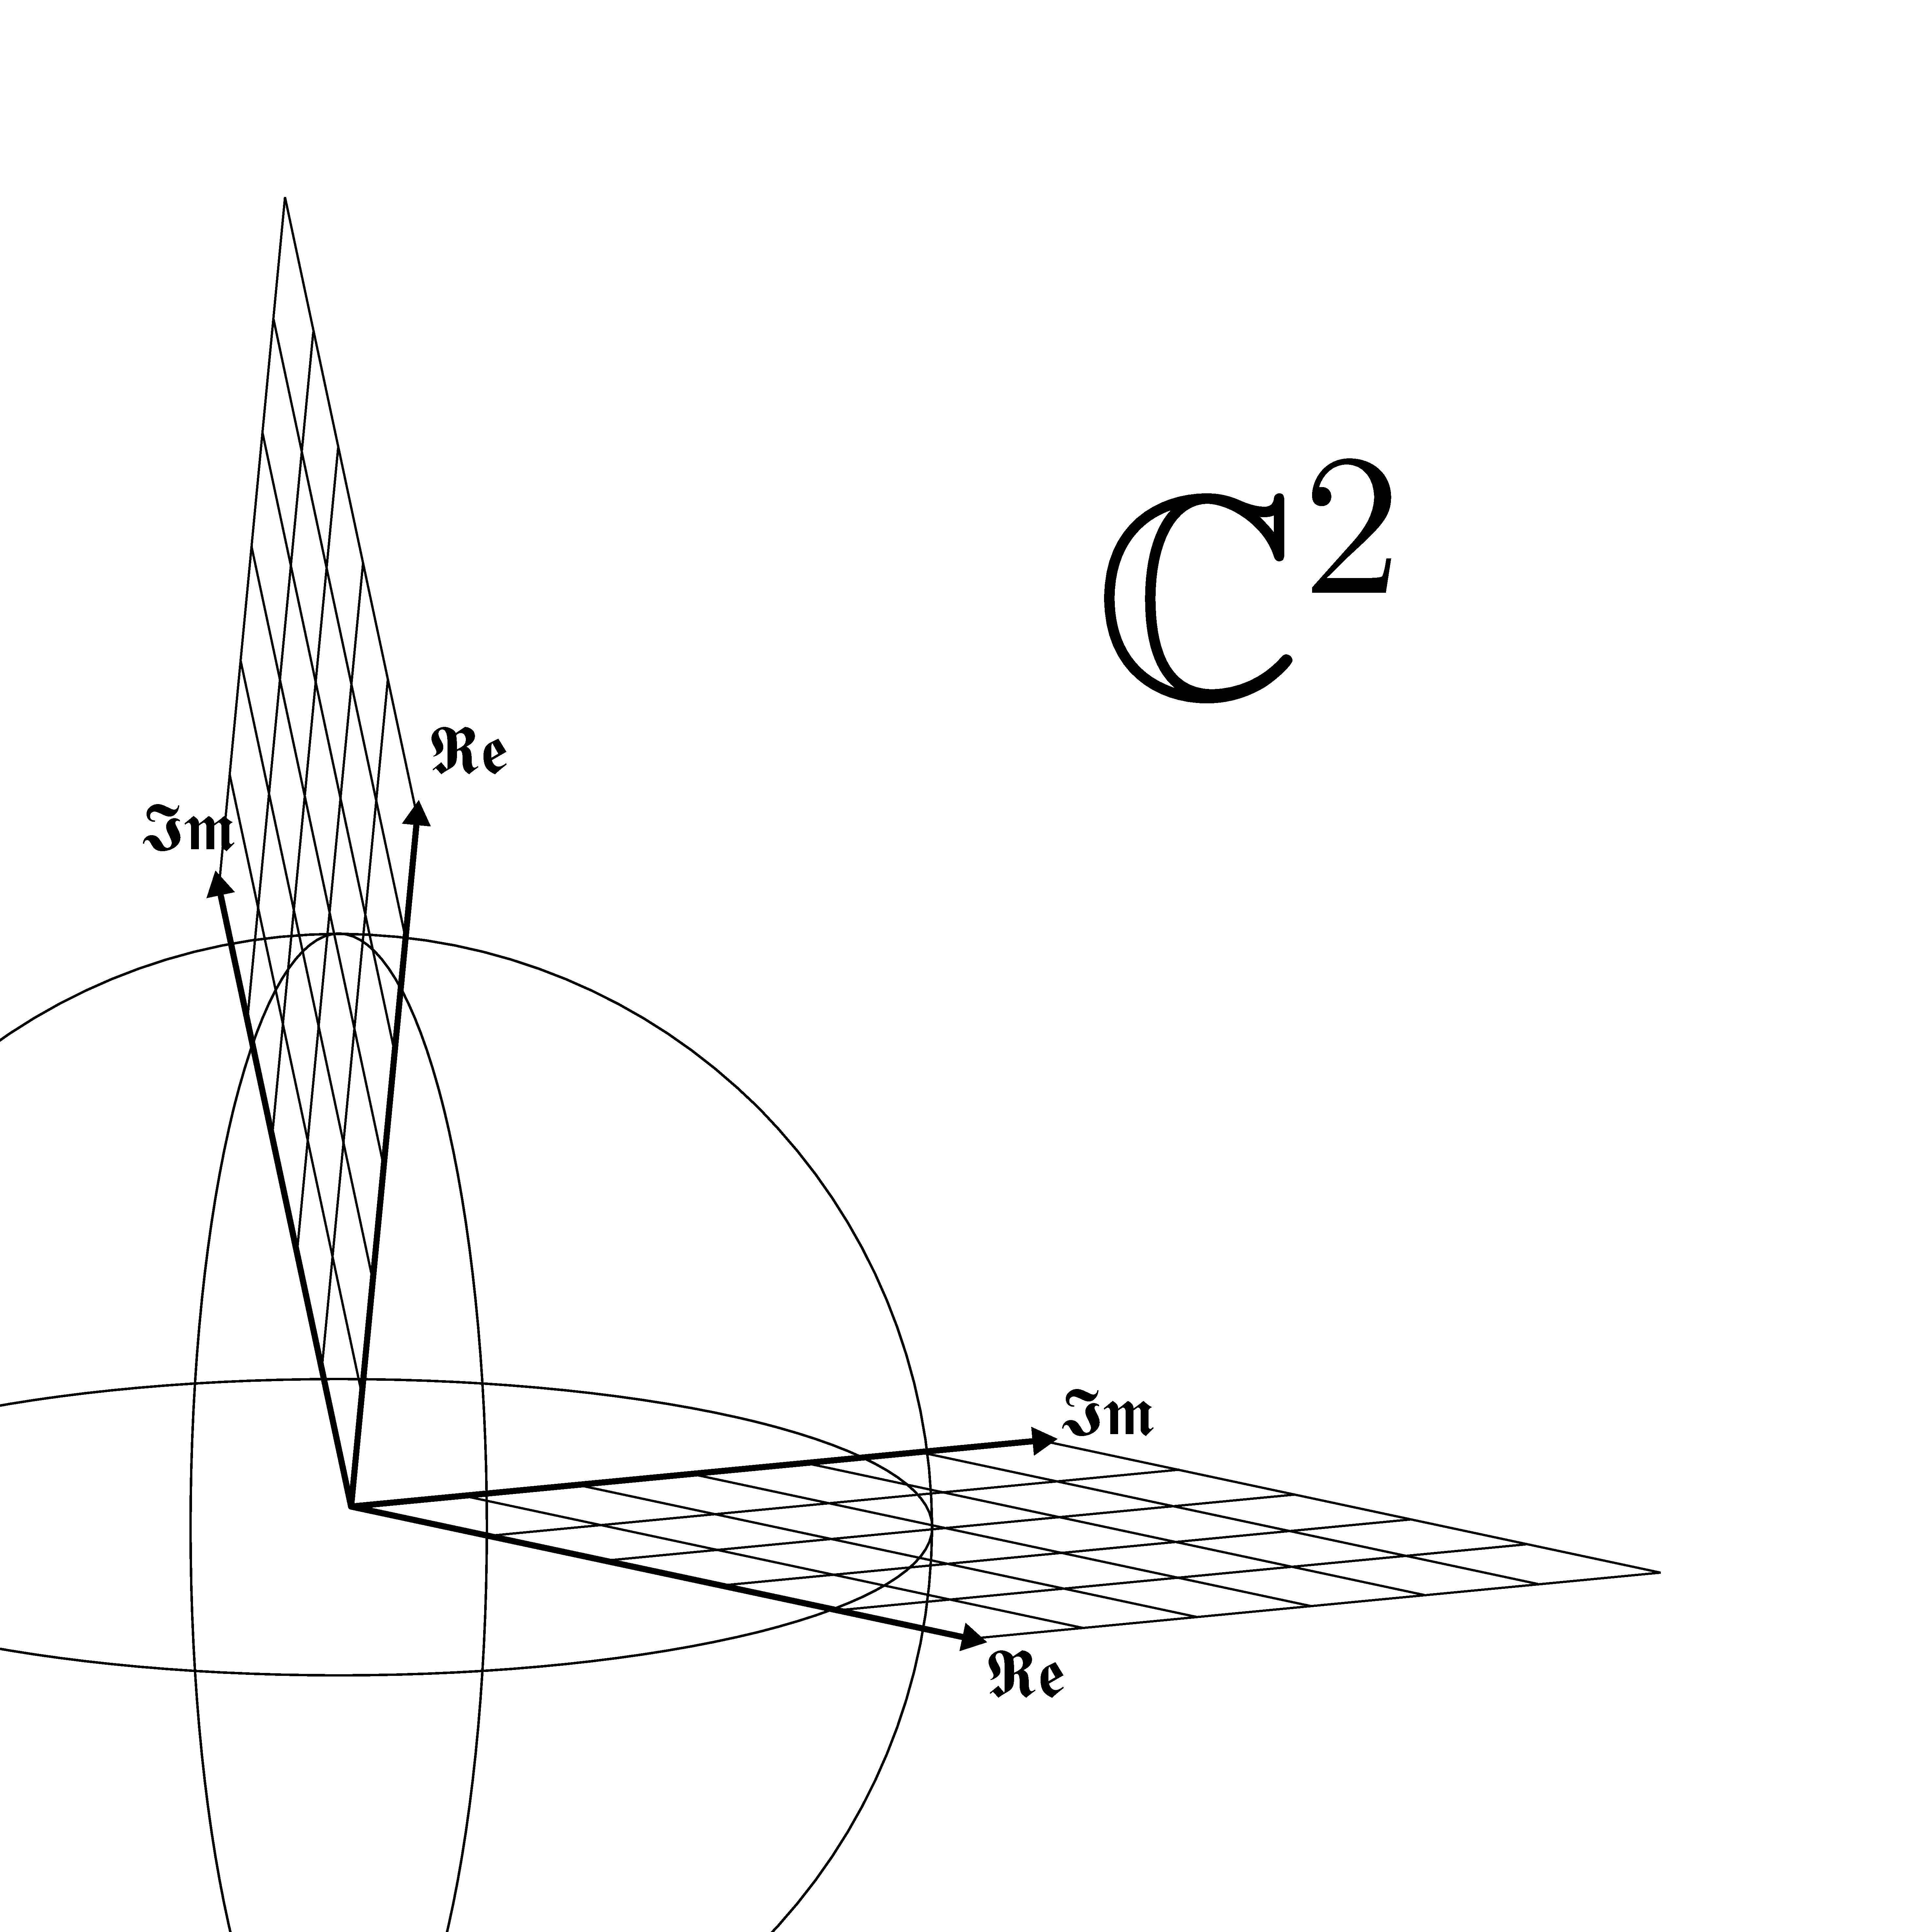
\includegraphics[width=6cm]{c2-sphere.pdf}
		\end{figure}
	\end{frame}

	\begin{frame}{\subsecname}
		\postulado{Composição}
		Um sistema é descrito pela composição dos estados que o representam, que se dá através do \emph{produto tensorial}.
		$\ket{\Psi} \otimes \ket{\Phi} \equiv \ket{\Psi\Phi}$
		
		\definicao{Produto de Kronecker}
		
		\begin{align*}
		\vetor{a}{b} \otimes \vetor{x}{y} = \vetor{a \vetor{x}{y}}{b \vetor{x}{y}} = \vetorx{ax}{ay}{bx}{by}
		\end{align*}
	\end{frame}
	
	\begin{frame}{\subsecname}
		\definicao{Base Computacional}
		A \emph{Base Computacional} é determinada pelos estados ortogonais $\ket{0}$ e $\ket{1}$, definidos por
		\begin{align*}
		\ket{0} &= \vetor{1}{0}\\
		\ket{1} &= \vetor{0}{1}\\
		\end{align*}
		Chamaremos estes estados de \textit{qubits}!
	\end{frame}
	
	
	
	\begin{frame}{\subsecname}
		\definicao{Base Computacional}
		A \emph{Base Computacional} é determinada pelos estados ortogonais $\ket{0}$ e $\ket{1}$, definidos por:
		\begin{align*}
		\ket{0} &= \vetor{1}{0}\\
		\ket{1} &= \vetor{0}{1}\\
		\end{align*}
	\end{frame}
	
	\begin{frame}{\subsecname}
		\postulado{Evolução}
		A evolução de um sistema se dá por meio de operadores unitários $U$
	\end{frame}
	
	\begin{frame}{\subsecname}
		\textbf{Uma nota sobre reversibilidade}
		
		$$\Delta S > K T \log 2$$
	\end{frame}
	
	\subsection{Trapped-ion}
	\begin{frame}{\subsecname}
		Oi íon aprisionado
	\end{frame}

	\subsection{Algoritmos}
	
	\begin{frame}{Algoritmo de Grover}
	
	\person{grover.jpg}{Lov Grover}{Bell Labs}{3cm}{2cm}{2cm}
		
	\end{frame}

	\begin{frame}{Algoritmo de Shor}
	
	\person{shor.jpg}{Peter Shor}{MIT}{3cm}{2cm}{2cm}
			
	\end{frame}
	

	\subsection{Teletransporte Quântico}
	
	\comicw{quantum-teleportation.pdf}
	
	\begin{frame}{\subsecname}
	
	\end{frame}
	
	\subsection{Teorema da não-clonagem}
	
	
	\begin{frame}{\subsecname}
	
	\teorema{Não-Clonagem}
		Não é possível fazer uma cópia de um estado quântico.
	\end{frame}
	
	\begin{frame}{\subsecname}
	\prova
	Vamos supor que existe um operador unitário $U$ capaz de clonar um estado $\ket{\Psi(t)} = \alpha \ket{\uparrow} + \beta \ket{\downarrow}$ qualquer, isto é:
		\begin{align*}
			U (\ket{\Psi} \otimes \ket{\xi}) = \ket{\Psi} \otimes \ket{\Psi}
		\end{align*}
	Assim:
		\begin{align*}
			\ket{\Psi} \otimes \ket{\xi} &= (\alpha \ket{\uparrow} + \beta \ket{\downarrow}) \otimes \ket{\xi}\\
			&= \alpha \ket{\uparrow} \otimes \ket{\xi} + \beta \ket{\downarrow} \otimes \ket{\xi}
		\end{align*}
		\begin{align*}
			\therefore U(\ket{\Psi} \otimes \ket{\xi}) &= U(\alpha \ket{\uparrow} \otimes \ket{\xi} + U(\beta \ket{\downarrow} \otimes \ket{\xi})\\
			&= \alpha U(\ket{\uparrow} \otimes \ket{\xi}) + \beta U(\ket{\downarrow} \otimes \ket{\xi})\\
			&= \alpha \ket{\uparrow} \otimes \ket{\uparrow} + \beta \ket{\downarrow} \otimes \ket{\downarrow}
		\end{align*}
	\end{frame}
	
	\begin{frame}{\subsecname}
	Por outro lado:
		\begin{align*}
		\ket{\Psi} \otimes \ket{\Psi} =& (\alpha \ket{\uparrow} + \beta \ket{\downarrow}) \otimes (\alpha \ket{\uparrow} + \beta \ket{\downarrow})\\
		=& \alpha^2 \ket{\uparrow\uparrow} + \alpha\beta (\ket{\uparrow\downarrow} + \ket{\downarrow\uparrow}) + \beta^2 \ket{\downarrow\downarrow}
		\end{align*}
	\end{frame}	
	
	\subsection{Fótons}	
	
	\begin{frame}{\subsecname}
		\imgw{superposition.pdf}{\textwidth}
	\end{frame}
	
	\subsection{Caminhadas Quânticas}
	
	\begin{frame}{\subsecname}
		\imgw{superposition.pdf}{\textwidth}
	\end{frame}

	\section{Computação Topológica}
	
	\subsection{Nós}
	
	\begin{frame}{\subsecname}
	
	\end{frame}	
	
	\begin{frame}{\subsecname}
	
	\end{frame}
	
	\subsection{Ânions}
	
	\begin{frame}{\subsecname}
	
	\end{frame}	
	
	\begin{frame}{\subsecname}
	
	\end{frame}
	
	\section{Computação Adiabática}
	
	\subsection{Teorema Adiabático}
	
	\begin{frame}{\subsecname}
		
		\begin{align*}
			H \ket{\Psi(t)} =\mathbbm{i} \hslash \frac{\partial \ket{\Psi(t)}}{\partial t}
		\end{align*}
	\end{frame}
	
	\begin{frame}{\subsecname}
	
	\end{frame}	
	
	\begin{frame}{\subsecname}
	
	\end{frame}
	
	\begin{frame}{\subsecname}
	
	\end{frame}
	
	\subsection{Têmpera Quântica}	
	
	\begin{frame}{\subsecname}
		\begin{align*}
			H(t) = &-\frac{A(t)}{2}  \sum_{i} h_i \cdot X\ket{s_i}\\ &+ \frac{B(t)}{2}\left(\sum_{i} h_i \cdot Z\ket{s_i} + \sum_{i < j} J_{i,j} \cdot Z\ket{s_i} \otimes Z\ket{s_j}\right)
		\end{align*}
	\end{frame}
	
	\begin{frame}{\subsecname}
		\imgw{energy-levels.pdf}{7cm}
	\end{frame}
	
	\subsection{Saltos Quânticos}
	
	\begin{frame}
	
	\end{frame}	
	
	\section{Fim?}

	
	\subsection{Material}
	
	\begin{frame}{\subsecname}
	
	\end{frame}
	
	\subsection{Bibliografia}
	
	\begin{frame}{\subsecname}
		\thebibliography{99}
		
		\bibitem{field:2018} \textbf{Introduction to topological quantum computation with non-Abelian anyons}, FIELD, B. \& SIMULA, T., School of Physics and Astronomy, Monash University, Victoria 3800, Australia.
		
		\bibitem{}
	\end{frame}
\end{document}